\documentclass[12pt]{jsarticle}
\usepackage[dvipdfmx]{graphicx}
\textheight = 25truecm
\textwidth = 18truecm
\topmargin = -1.5truecm
\oddsidemargin = -1truecm
\evensidemargin = -1truecm
\marginparwidth = -1truecm


\def\theenumii{\Alph{enumii}}
\def\theenumiii{\alph{enumiii}}
\def\labelenumi{(\theenumi)}
\def\labelenumiii{(\theenumiii)}
\def\theenumiv{\roman{enumiv}}
\def\labelenumiv{(\theenumiv)}
\usepackage{comment}
\usepackage{url}

%%%%%%%%%%%%%%%%%%%%%%%%%%%%%%%%%%%%%%%%%%%%%%%%%%%%%%%%%%%%%%%%
% sty/ にある研究室独自のスタイルファイル
\usepackage{jtygm}  % フォントに関する余計な警告を消す
\usepackage{nutils} % insertfigure, figref, tabref マクロ

\def\figdir{./figs} % 図のディレクトリ
\def\figext{pdf}    % 図のファイルの拡張子


\begin{document}
%%%%%%%%%%%%%%%%%%%%%%%%%%%%
%% 表題
%%%%%%%%%%%%%%%%%%%%%%%%%%%%
\begin{center}
{\LARGE SlackBotプログラムの仕様書}
\end{center}

\begin{flushright}
  2020/7/21\\
  野村 優文
\end{flushright}
%%%%%%%%%%%%%%%%%%%%%%%%%%%%
%% 概要
%%%%%%%%%%%%%%%%%%%%%%%%%%%%

\section{概要}\label{sec:overview}
\label{sec:introduction}
本資料は,2020年度新人研修課題で作成したSlackBotプログラムの仕様をまとめたものである.
本プログラムではチャットツールであるSlack\cite{Slack}を用いる.
また,SlackBotは,SlackクライアントがSlack上で投稿した特定の文章をきっかけとして,Slack上で自動的に返信する機能をもつ.
本プログラムは以下の2つの機能をもつ.

\begin{description}
\item[(機能1)] Slackクライアントから指定された文字列を返信する機能
  
\item[(機能2)]\label{enum:function2} %Weather Hacks(気象データ配信サービス)\cite{Weather_Hacks}を用いて
  天気予報の情報を返信する機能
\end{description}

\section{対象とする利用者}
本プログラムでは,Slackアカウントを所有する利用者を対象としている.


\section{SlackBotプログラムの処理の流れ}
\label{sec:flow}
%\subsection{概要}
%本プログラムの処理の流れを以下に機能別に記述する.
%本章では,本プログラムの処理の流れを記述する.

\subsection{(機能1)の処理の流れ}
(機能1)の処理の流れを図\ref{fig:slackbot_flow}に示し,以下で各処理について説明する.
  \begin{figure}[t]
    \centering
    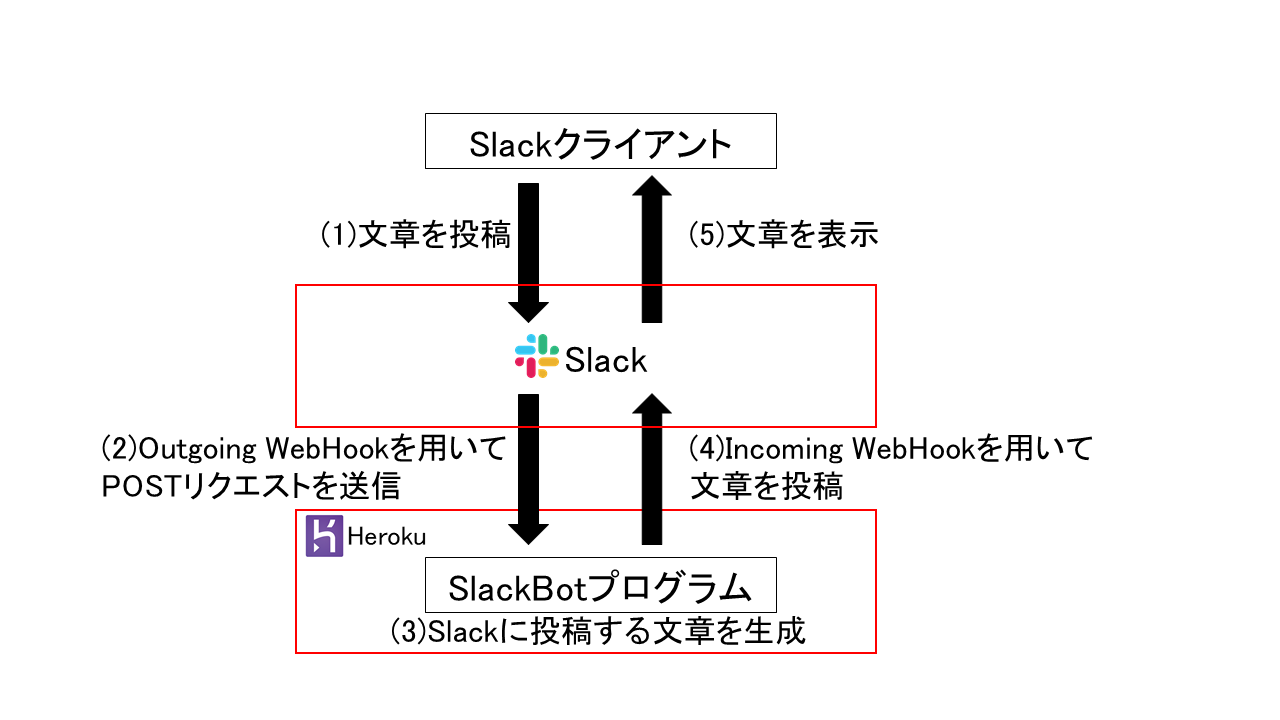
\includegraphics[width=1\textwidth]{figs/slackbot_flow12.png}
    \caption{Slackクライアントから指定された文字列を返信する機能の処理の流れ}
    \label{fig:slackbot_flow}
  \end{figure}

\begin{enumerate}
\item SlackクライアントがSlackへ文章を投稿する.
\item SlackはOutgoing WebHookを用いて,%Slackクライアントが投稿した文章を
  SlackBotプログラムにPOSTリクエストを送信する.
  Outgoing WebHookとは,特定の文章がSlackに投稿されたとき,この特定の文章や投稿したSlackクライアントなどの情報を含んで,指定したURLにPOSTリクエストを送信する機能である.
%\item\label{enum:request} SlackBotプログラムはWebサービスにリクエストを送信する.
%\item\label{enum:response} Webサービスは,リクエストの内容に応じてSlackBotプログラムにレスポンスを送信する.
\item Heroku上で動作するSlackBotプログラムは,Slackに投稿する文章を生成する.
  Herokuとは,プログラムをデプロイすることにより,クラウド上でプログラムを実行することができるプラットフォームである.
\item SlackBotプログラムは,Incoming WebHookを用いて,生成した文章をSlackに投稿する.
  Incoming WebHookとは,外部のサービスからSlackに文章を投稿する機能である.
\item Slackは,SlackBotプログラムが投稿した文章を表示する.
\end{enumerate}

\subsection{(機能\ref{enum:function2})の処理の流れ}
(機能\ref{enum:function2})の処理の流れを図\ref{fig:slackbot_flow2}に示し,以下で各処理について説明する.
  \begin{figure}[t]
    \centering
    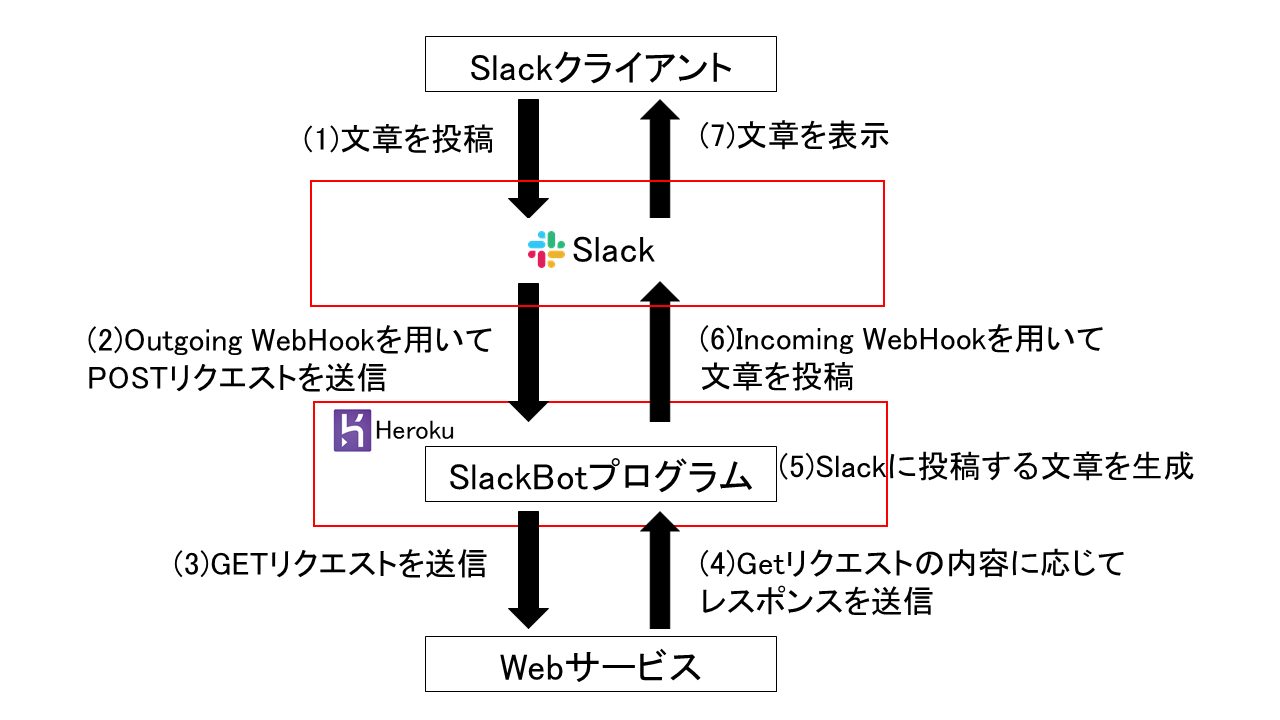
\includegraphics[width=1\textwidth]{figs/slackbot_flow13.png}
    \caption{天気予報の情報を返信する機能の処理の流れ}
    \label{fig:slackbot_flow2}
  \end{figure}

%図\ref{fig:slackbot_flow}より,Incoming WebHookとは,外部のサービスからSlackに文章を投稿する機能である.
%Outgoing WebHookとは,特定の文章がSlackに投稿されたとき,指定したURLにこの特定の文章をPOSTする機能である.
%Herokuとは,プログラムをデプロイすることにより,クラウド上でプログラムを実行することができるプラットフォームである.
%本プログラムは,機能を利用するために,上記の2つのWebHookおよびHerokuの設定を行う必要がある.
\begin{enumerate}
\item SlackクライアントがSlackへ文章を投稿する.
\item SlackはOutgoing WebHookを用いて,%Slackクライアントが投稿した文章を
  SlackBotプログラムにPOSTリクエストを送信する.
%  Outgoing WebHookとは,特定の文章がSlackに投稿されたとき,指定したURLにこの特定の文章をPOSTする機能である.
\item\label{enum:request} SlackBotプログラムはWebサービスにGETリクエストを送信する.
\item\label{enum:response} Webサービスは,GETリクエストの内容に応じて,SlackBotプログラムにレスポンスを送信する.
\item Heroku上で動作するSlackBotプログラムは,Webサービスからのレスポンスを元にして,Slackに投稿する文章を生成する.
\item SlackBotプログラムは,Incoming WebHookを用いて,生成した文章をSlackに投稿する.
%  Incoming WebHookとは,外部のサービスからSlackに文章を投稿する機能である.
\item Slackは,SlackBotプログラムが投稿した文章を表示する.
\end{enumerate}

%本プログラムの\ref{sec:overview}章(\ref{enum:function2})の機能を使用しないときは,(\ref{enum:request})(\ref{enum:response})の処理を省略する.

\section{機能}\label{sec:function}
SlackクライアントがSlack上に``@masabot''で始まる文章を投稿したとき,本プログラムは受け取った文字列に対応する文章をSlack上に返信する.
本プログラムが返信する文章は,Slackクライアントが投稿する``@masabot''の後ろに付く文字列によって決まる.
以下に本プログラムがもつ機能について記述する.
\begin{description}
\item[(機能1)] Slackクライアントから指定された文字列を返信する機能
  
  この機能は,Slackクライアントが``@masabot 「(指定した文字列)」と言って''と投稿したとき,SlackBotプログラムは``「''と``」と言って''の間にある文字列を読み込んで,``(指定した文字列)''という文章を返信する.
  例えば,Slackクライアントが``@masabot 「こんにちは」と言って''と投稿したとき,Slackbotは``こんにちは''と返信する.
  ただし,``(指定した文字列)''の中に``「'',もしくは``」''を含んではならない.

\item[(機能2)]\label{func2}  %Weather Hacks(気象データ配信サービス)を用いて
  天気予報の情報を返信する機能

  この機能は,Slackクライアントが``@masabot (日にち)の(都道府県名)の天気''と投稿したとき,指定した``(日にち)''における``(都道府県名)''の天気予報の情報を返信する.
%  この情報を返信するために,Weather Hacks(気象データ配信サービス)を用いている.
  例として,Slackクライアントが``@masabot 明日の東京都の天気''と投稿したときの,SlackBotの返信を図\ref{fig:weather}に示す.
  \begin{figure}[t]
    \centering
    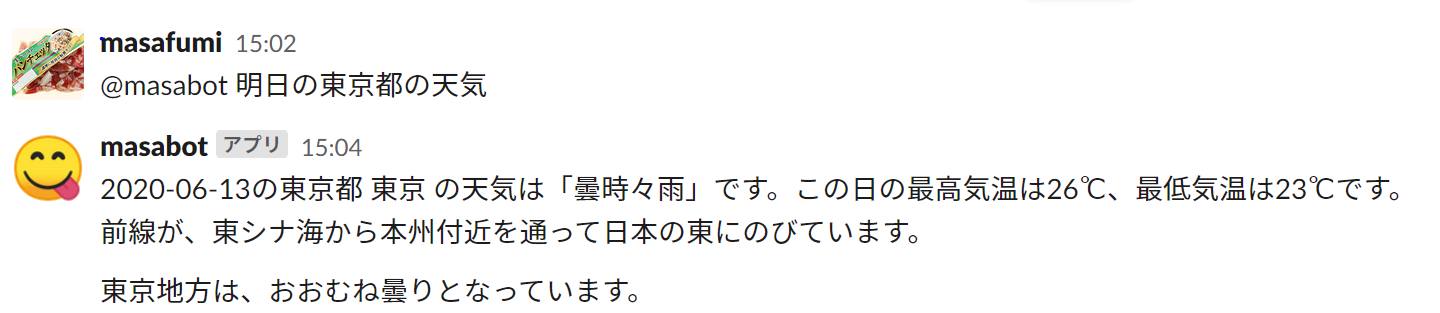
\includegraphics[width=1\textwidth]{figs/slackbot_weather2.png}
    \caption{Slackクライアントが``@masabot 明日の東京都の天気''と投稿したときの,SlackBotの返信}
    \label{fig:weather}
  \end{figure}
  この機能を使用するにあたって,Slackクライアントが指定できる``(日にち)''と``(都道府県名)''を表\ref{tab:3}に示す.
  \begin{table}[t]
  \begin{center}
    \caption{指定できる``(日にち)''と``(都道府県名)''}\label{tab:3}
%    \ecaption{Operating environment.}
    \begin{tabular}{l|l|l}
      \hline\hline
      \multicolumn{1}{l|}{項目} & \multicolumn{1}{l}{内容} &\multicolumn{1}{|l}{備考}\\
      \hline
      ``(日にち)'' & ``今日'',``明日'',``明後日'' &\\
      ``(都道府県名)'' & 47都道府県名のいずれか1つ & ``都'',``府'',および``県''は省略可\\
      \hline
    \end{tabular}
  \end{center}
  \end{table}
  Slackクライアントは,表\ref{tab:3}から``(日にち)''に入れる文字列を1つ指定する.
  また, ``(都道府県名)''には,47都道府県から都道府県名を1つ指定する.
  これらの情報を用いて,SlackクライアントはSlackに``@masabot (日にち)の(都道府県名)の天気''と投稿する.
  これにより,SlackBotは指定された``(日にち)''における``(都道府県名)''の天気予報の情報を返信する.
  このときに返信する天気予報の情報は,WebサービスであるWeather Hacks(気象データ配信サービス)\cite{Weather_Hacks}を利用して取得している.
%また,Slackクライアントは ``(都道府県名)''を指定する際, ``都'',``府'',``県''という文字を省略してSlackに投稿しても,SlackBotは指定された ``(都道府県名)''の天気予報の情報を返信することができる. 
\end{description}

Slackクライアントが(機能1),(機能2)のどちらにも当てはまらない文章をSlackに投稿したとき,本プログラムは以下の文章を返信する.
\begin{verbatim}
   こんにちは、masabotです。        
   "@masabot 「○○○」と言って"と投稿した場合、"○○○"と返信します。
   天気予報を知りたいときは、"@masabot □□の△△の天気" 
   (□□は「今日」「明日」「明後日」のいずれか)(△△は都道府県名) と投稿してください。
   この日の指定した都道府県の天気を返信します。
\end{verbatim}

\section{動作環境}\label{sec:environment}
本プログラムはHeroku上で動作する.
%Herokuとは,プログラムをデプロイすることにより,クラウド上でプログラムを実行することができるプラットフォームである.
Herokuの動作環境を表\ref{tab:2}に示す.
\begin{table}[t]
  \begin{center}
    \caption{動作環境}\label{tab:2}
%    \ecaption{Operating environment.}
    \begin{tabular}{l|l}
      \hline\hline
      \multicolumn{1}{l|}{項目} & \multicolumn{1}{l}{内容}\\
      \hline
      OS & Ubuntu 18.04.4 LTS\\
      CPU & Intel(R) Xeon(R) CPU E5-2670 v2 @ 2.50GHz\\
      メモリ & 512MB\\
      Ruby & ruby 2.6.6p146\\
      Gem & activesupport 6.0.2.2\\
     & bundler 2.0.2\\
     & mustermann 1.1.1\\
     & rack 2.2.2\\
     & rack-protection 2.0.8.1\\
     & ruby2\_keywords 0.0.2\\ 
     & sinatra 2.0.8.1\\
     & tilt 2.0.10\\
      \hline
    \end{tabular}
  \end{center}
\end{table}

\section{環境構築}

\subsection{概要}
本プログラムを動作させるための環境の構築手順を以下に記述する.
\begin{enumerate}
\item SlackのIncoming WebHookの設定
\item SlackのOutgoing WebHookの設定
\item Herokuアカウントの作成と設定
\end{enumerate}

上記の構築手順の詳細を以下に記述する.

\subsection{SlackのIncoming WebHookの設定}\label{sec:Incoming}
SlackにおけるIncoming WebHookの設定を以下の手順で行う.
\begin{enumerate}
\item 自分のSlackアカウントにログインする.
\item Slackの左上のメニューを開き,「その他管理項目」の「アプリを管理する」を開く.
\item カスタムインテグレーションから,「Incoming WebHook」を開く.
\item 「Slackに追加」を選択した後,Incoming WebHookがメッセージを投稿するチャンネルを選択し,インテグレーションを追加する.
\item\label{enum:Heroku_URL} 「名前をカスタマイズ」にて,設定するIncoming WebHookの名前を入力する.
  また,WebHook URLを\ref{sec:setup_Heroku}節(\ref{enum:in_URL})で使用するので控えておく.
\item 「設定を保存する」を選択する.
\end{enumerate}

\subsection{SlackのOutgoing WebHookの設定}
SlackにおけるOutgoing WebHookの設定を以下の手順で行う.
\begin{enumerate}
\item 自分のSlackアカウントにログインする.
\item Slackの左上のメニューを開き,「その他管理項目」から「アプリを管理する」を開く.
\item カスタムインテグレーションから,「Outgoing WebHook」を開く.
\item 「インテグレーションを追加する」を選択する.
\item Outgoing WebHookに関して,以下の設定を行う.
  \begin{enumerate}
  \item 「チャンネル」にて,Slackクライアントが投稿した特定の文字列を監視するチャンネルを設定する.
  \item 「引き金となる言葉」にて,WebHookが動作する契機となる文字列を入力する.
  \item 「名前をカスタマイズ」にて,設定するOutgoing WebHookの名前を入力する.
  \end{enumerate}
\item 「設定を保存する」を選択する.
\end{enumerate}

\subsection{Herokuアカウントの作成と設定}\label{sec:setup_Heroku}
Herokuアカウントの作成と設定を以下の手順で行う.
\begin{enumerate}
\item 以下のURLよりHerokuにアクセスし,「新規登録」よりHerokuアカウントを登録する.
\begin{verbatim}
  https://jp.heroku.com/
\end{verbatim}
\item 登録したアカウントでログインし,「Getting Started on Heroku」にて,「Ruby」を選択する.
\item 以下のコマンドを実行し,Heroku CLIをインストールする.
\begin{verbatim}
  $ sudo snap install heroku --classic
\end{verbatim}
\item \verb|heroku|コマンドを使用するために,以下のコマンドを実行し,パスを通す.
\begin{verbatim}
  $ export PATH=$PATH:/snap/bin/
\end{verbatim}
\item 以下のコマンドを実行し,Heroku CLIがインストールできていることを確認する.
\begin{verbatim}
  $ heroku version
  heroku/7.42.0 linux-x64 node-v12.16.2
\end{verbatim}
上記の例では,\verb|heroku/7.42.0 linux-x64 node-v12.16.2|のHeroku CLIがインストールできていることを示している.

\item 以下のコマンドを実行し,Heroku CLIにログインする.
\begin{verbatim}
  $ heroku login
\end{verbatim}

\item\label{enum:app} 作成したアプリケーションのディレクトリに移動して,以下のコマンドを実行し,Heroku上にアプリケーションを生成する.
\begin{verbatim}
  $ heroku create <myapp_name>
\end{verbatim}
\verb|<myapp_name>|にはアプリケーション名を入力する.
なお,アプリケーション名は小文字,数字,およびハイフンのみ使用できる.

\item 以下のコマンドを実行し,生成したHerokuのアプリケーションが,登録されていることを確認する.
\begin{verbatim}
    $ git remote -v
    heroku	https://git.heroku.com/<myapp_name>.git (fetch)
    heroku	https://git.heroku.com/<myapp_name>.git (push)
\end{verbatim}
\item\label{enum:in_URL} 以下のコマンドを実行し,\ref{sec:Incoming}節(\ref{enum:Heroku_URL})で控えておいたIncoming WebHook URLを,Herokuの環境変数に追加する.
\begin{verbatim}
  $ heroku config:set INCOMING_WEBHOOK_URL="https://XXXXXXXXXXXX"
\end{verbatim}
上記のコマンドにおける\verb|"https://XXXXXXXXXXXX"|に,\ref{sec:Incoming}節(\ref{enum:Heroku_URL})で控えておいたIncoming WebHook URLを入力する.
\end{enumerate}

\section{使用方法}
本プログラムを使用するには,以下の手順で行う.
\begin{enumerate}
\item 以下に示すGitリポジトリから本プログラムを取得する.
\begin{verbatim}
  git@github.com/masafumi0612/BootCamp.git
\end{verbatim}
本プログラムは,上記のGitリポジトリ内の\verb|2020/SlackBot/SlackBot.rb|及び,\verb|2020/SlackBot/MySlackBot.rb|である.

\item 以下のコマンドを用いて,本プログラムをHerokuにデプロイする.
\begin{verbatim}
  $ git push heroku master
\end{verbatim}
\end{enumerate}

\section{エラー処理}
本プログラムにおけるエラー処理を以下に記述する.
\begin{enumerate}
\item (機能2)を使用する際に,Slackクライアントが投稿する文字列の中に(日にち)が含まれていないときや,使用できる``今日'',``明日''および``明後日''以外の文字列を使用したときは,``今日''の指定した都道府県の天気予報を返信する.
  例えば,``東京都の天気''や``明々後日の東京都の天気''という文字列を投稿した際は,今日の東京都の天気予報を返信する.

  \item (機能2)を使用する際に,Slackクライアントが投稿する文字列の中に都道府県名が含まれていないとき,本プログラムは以下のように返信する.
\begin{verbatim}
   都道府県名を入力してください。
   天気予報を知りたいときは、"@masabot □□の△△の天気" 
   (□□は「今日」「明日」「明後日」のいずれか)(△△は都道府県名) と投稿してください。
   指定した日にちの都道府県の天気を返信します。
\end{verbatim}
これに当てはまる例として,Slackクライアントが``@masabot 明日の天気''という文字列を投稿したときが挙げられる.
\end{enumerate}

\section{保証しない動作}
本プログラムの保証しない動作を以下に記述する. 
\begin{enumerate}
\item \ref{sec:environment}章に示した動作環境以外の環境で,本プログラムを実行したときの動作
\item 本プログラムが,SlackのOutgoing WebHook以外からPOSTリクエストを受け取って実行した際の動作
  
\end{enumerate}

\bibliographystyle{ipsjunsrt}
\bibliography{mybibdata}

\end{document}
